\documentclass[11pt,a4paper]{article}
\usepackage[utf8]{inputenc}
\usepackage[T1]{fontenc}
\usepackage{amsmath}
\usepackage{amsfonts}
\usepackage[francais]{babel}
\usepackage{amssymb}
\usepackage{graphicx}
\usepackage[top=2.00cm]{geometry}
\usepackage{enumitem}
\usepackage{tikz}
\usepackage{mathtools}
\usepackage{pgfplots}
\usetikzlibrary{plotmarks}
\usepackage{bigcenter}
\usepackage{multicol}
\date{21 octobre 2016}
%Modif des enumerates numeros en gras. leftmargin=*,
\setlist[enumerate]{label=\textbf{\arabic*}.}

\usepackage{titlesec}
%modif des titres de section diminuer la taille
\titleformat{\section}
  {\normalfont\fontsize{14}{15}\bfseries}{\thesection}{1em}{}
\titleformat{\subsection}
  {\normalfont\fontsize{12}{15}\bfseries}{\thesubsection}{1em}{}


\author{CHARNAY Valentin, FINOT Sylvain}
\title{Compte rendu de TP : \\ Les Amplificateurs Opérationnels}

\begin{document}
\maketitle
\section{Montage AMPLIFICATEUR NON INVERSEUR, ET SES LIMITATION EN FRÉQUENCE}

Dans ce TP, les mesures de tension faites sont toutes sauf indication en "crête à crête" .

\subsection{Étude du montage à basse fréquence (Amplificateur Opérationnel considéré idéal)}
%Premiere partie (2.1)
\begin{enumerate}
\item Nous voulons obtenir un gain en tension de 50. Avec le montage que nous avons, nous trouvons que : 
\begin{align}
v_{+}&=v_{e}\\
v_{-}&=\dfrac {R_{1}} {R_{1}+R_{2}}v_{s}
\end{align}
On trouve la relation (2) grâce à une loi des mailles, $v_{-}$ n'est autre que la tension aux bornes de $R_{1}$, c'est un pont diviseur de tension. \\
En considérant que l'amplificateur est idéal, cela implique qu'il n'y ait pas de tension entre ses bornes et donc que la différence de potentiel est nulle.
\begin{align*}
v_{+}-v_{-}&=0 \iff v_{+}=v_{-} \\
\iff v_{e}&=\dfrac {R_{1}} {R_{1}+R_{2}}v_{s}
\end{align*}
On trouve alors la relation suivante :
\begin{align*}
G\equiv\dfrac{v_{s}}{v_{e}}=\dfrac {R_{1}+R_{2}} {R_{1}}=1+\dfrac {R_{2}} {R_{1}}
\end{align*}
On cherche donc deux résistances telles que $G=50 \implies \dfrac {R_{2}} {R_{1}}=49$ \\
Nous nous sommes rapproché de cette valeur en prenant \\ $R_{1}=1k\varOmega$ et $R_{2}=47k\varOmega$. Les résistances que nous avons choisi ont une précision de 5\%, ainsi :
\begin{align*}
G&=1+\dfrac{47}{1}=48\\
\Delta G&=G\sqrt {\left( \dfrac {\Delta R_{1}} {R_{1}}\right) ^{2}+\left( \dfrac {\Delta R_{2}} {R_{2}}\right) ^{2}}\\
&\approx 48\sqrt { 0.05^{2}+0.05 ^{2}} \approx 3,4 \\
\implies G& \approx 48\pm3,4
\end{align*}

Expérimentalement nous avons mesuré $v_{e}$ et $v_{s}$ crête à crête en prenant en compte les incertitudes de lecture sur l'oscilloscope. Estimation de l'incertitude : une graduation (un cinquième de division). Il a fallu également choisir $v_{e}$ suffisamment petit pour ne pas être en régime saturé (i.e $v_{e}<\dfrac{v_{sat}}{G}$)
\begin{align*}
v_{e}&=0,4\pm 2.10^{-2}V \qquad v_{s}=20\pm1V \qquad G=\dfrac{v_{e}}{v_{s}}\approx \dfrac{20}{0,4}\approx 50\\
\Delta G&=G\sqrt {\left( \dfrac {\Delta v_{e}} {v_{e}}\right) ^{2}+\left( \dfrac {\Delta v_{s}} {v_{s}}\right) ^{2}}\\
&\approx 50\sqrt {\left( \dfrac {2.10^{-2}} {0,4}\right) ^{2}+\left( \dfrac {1} {20}\right) ^{2}}\approx 3,5
\end{align*}

\item On refait de même en faisant varier $R_{2}$, seul l'application numérique diffère.
\begin{itemize}

\item Pour $R_{2}'=100k\Omega$, théoriquement on trouve :
\begin{align*}
G'&=1+\dfrac{100}{1}=101\\
\Delta G'&=G'\sqrt {\left( \dfrac {\Delta R_{1}} {R_{1}}\right) ^{2}+\left( \dfrac {\Delta R_{2}'} {R_{2}'}\right) ^{2}}\\
&\approx 101\sqrt { 0.05^{2}+0.05 ^{2}} \approx 7,1 \\
\implies G'&\approx 101 \pm7,1
\end{align*}

Expérimentalement :
\begin{align*}
v_{e}'&=0,1\pm 10^{-2}V \qquad v_{s}'=10,4\pm0,4V \qquad G'=\dfrac{v_{e}'}{v_{s}'}\approx \dfrac{10,4}{0,1} \approx 104\\
\Delta G'&=G'\sqrt {\left( \dfrac {\Delta v_{e}'} {v_{e}'}\right) ^{2}+\left( \dfrac {\Delta v_{s}'} {v_{s}'}\right) ^{2}}\\
&\approx 104\sqrt {\left( \dfrac {10^{-2}} {0,1}\right) ^{2}+\left( \dfrac {0,4} {10,4}\right) ^{2}}\approx 11,14
\end{align*}


\item Pour $R_{2}''=22k\Omega$, théoriquement on trouve :
\begin{align*}
G''&=1+\dfrac{22}{1}=23\\
\Delta G''&=G''\sqrt {\left( \dfrac {\Delta R_{1}} {R_{1}}\right) ^{2}+\left( \dfrac {\Delta R_{2}''} {R_{2}''}\right) ^{2}}\\
&\approx 23\sqrt { 0.05^{2}+0.05 ^{2}}\approx 1,6 \\
\implies G''&\approx 23 \pm1,6
\end{align*}
Expérimentalement :
\begin{align*}
v_{e}''&=0,1\pm 10^{-2}V \qquad 
v_{s}''=2,4\pm0,1V \qquad 
G''=\dfrac{v_{e}''}{v_{s}''}\approx \dfrac{2,4}{0,1}\approx 24\\
\Delta G''&=G''\sqrt {\left( \dfrac {\Delta v_{e}''} {v_{e}''}\right) ^{2}+\left( \dfrac {\Delta v_{s}''} {v_{s}''}\right) ^{2}}\\
&\approx 24\sqrt {\left( \dfrac {10^{-2}} {0,1}\right) ^{2}+\left( \dfrac {0,1} {2,4}\right) ^{2}}\approx 2,6 \\
\implies G''&\approx 24\pm2,6
\end{align*}
\end{itemize}
\textbf{Conclusion}: Dans chacun des cas, la valeur obtenue par la mesure correspond à la valeur théorique calculé. On peut donc dire que l'approximation d'un amplificateur idéal est bonne.
\item A présent on garde $R_{2}$ fixe et nous faisons varier la fréquence pour étudier le comportement de l'amplificateur.
On remarque que le Gain devient quasi-nul.
\end{enumerate}

%(2.2)
\subsection{Étude en fréquence du gain G(j$f$) avec amplificateur réel}
\begin{enumerate}
\item Calcul du gain à voir (on a pas fait le cours dessus).
\item On cherche à tracer le diagramme de Bode : $G_{dB}=20 \log{(\left| G(jf)\right|)}$ en fonction de $\log{(f)}$.\\ A l'aide de Regressi on obtient :
%\begin{bigcenter}
%\begin{tabular}{|c|c|c|c|c|c|c|c|c|c|c|}
%i & $f$ & $v_{e}$ & $\Delta v_{e}$ & $v_{s}$ & $\Delta v_{s}$ & G & $\Delta G$ & $\log{(f)}$ & $G_{dB}$ & $\Delta G_{dB}$\cr
% & Hz & Hz & V & V & V & V &  &  &  & \cr
%0 & 1096  & 0,1000 & 0,0040 & 2,400 & 0,10 & 24,00 & 1,4 & 3,040  & 27,60 & 0,50\cr \newline
%1 & 6793  & 0,1040 & 0,0040 & 2,400 & 0,10 & 23,08 & 1,3 & 3,832  & 27,26 & 0,49\cr \newline
%2 & 1,272·10${^4}$  & 0,1080 & 0,0040 & 2,400 & 0,10 & 22,22 & 1,2 & 4,104  & 26,94 & 0,48\cr
%3 & 2,129·10${^4}$  & 0,1080 & 0,0040 & 2,400 & 0,10 & 22,22 & 1,2 & 4,328  & 26,94 & 0,48\cr
%4 & 2,742·10${^4}$  & 0,1080 & 0,0040 & 2,300 & 0,10 & 21,30 & 1,2 & 4,438  & 26,57 & 0,50\cr
%5 & 3,100·10${^4}$  & 0,1080 & 0,0040 & 2,300 & 0,10 & 21,30 & 1,2 & 4,491  & 26,57 & 0,50\cr
%6 & 4,507·10${^4}$  & 0,1200 & 0,0040 & 2,000 & 0,10 & 16,67 & 1,0 & 4,654  & 24,44 & 0,52\cr
%7 & 6,478·10${^4}$  & 0,1160 & 0,0040 & 1,700 & 0,10 & 14,66 & 1,0 & 4,811  & 23,32 & 0,59\cr
%8 & 9,598·10${^4}$  & 0,1160 & 0,0040 & 1,280 & 0,040 & 11,03 & 0,51 & 4,982  & 20,86 & 0,40\cr
%9 & 1,503·10${^5}$  & 0,1160 & 0,0040 & 0,8800 & 0,040 & 7,586 & 0,43 & 5,177  & 17,60 & 0,50\cr
%10 & 2,024·10${^5}$  & 0,1200 & 0,0040 & 0,6800 & 0,020 & 5,667 & 0,25 & 5,306  & 15,07 & 0,39\cr
%11 & 2,651·10${^5}$  & 0,1240 & 0,0040 & 0,5200 & 0,020 & 4,194 & 0,21 & 5,423  & 12,45 & 0,44\cr
%12 & 5,370·10${^5}$  & 0,1260 & 0,0040 & 0,2700 & 0,010 & 2,143 & 0,10 & 5,730  & 6,620 & 0,42\cr
%13 & 1,023·10${^6}$  & 0,1240 & 0,0040 & 0,1500 & 0,010 & 1,210 & 0,090 & 6,010  & 1,653 & 0,64\cr
%\end{tabular}
%\end{bigcenter}
%Nous avons constaté que la tension d'entrée $v_{e}$ variait un peu, nous l'avons donc relevée également.

\begin{bigcenter}
\begin{tikzpicture}
\begin{axis}[ 
height=8cm,width=16cm
,axis x line=bottom,axis y line=left
,xmin=2.81821477278792,xmax=5.58203577915185
,ymin=6.92393678068692,ymax=39.8062416578858
,grid=major
,title={$G_{dB}$ en fonction de $\log{(f)}$ pour différentes valeurs de $R_{2}$}
,xlabel={$\log{(f)}$}
,ylabel={$G_{dB}$}
,legend entries={$R_{2}=33$,$R_{2}=68$,$R_{2}=82$}
]
\addplot[draw=red
,smooth,dashed
,error bars/.cd,y dir=both, y explicit,x dir=both, x explicit,error mark=none
] table[x error index=2,y error index=3]
 {gain10.txt};
\addplot[draw=blue
,smooth
,error bars/.cd,y dir=both, y explicit,x dir=both, x explicit,error mark=none
] table[x error index=2,y error index=3]
 {gain12.txt};
\addplot[draw=orange
,smooth,dash pattern=on 4pt off 2pt on 1pt off 2pt
,error bars/.cd,y dir=both, y explicit,x dir=both, x explicit,error mark=none
] table[x error index=2,y error index=3]
 {gain14.txt};

\end{axis}
\end{tikzpicture}
\end{bigcenter}

On remarque qu'il y a une nette diminution du gain à partir d'une fréquence de seuil $f_{0}$.
Tant que la fréquence $f$ est inférieure à $f_{0}$ le gain est relativement proche du gain théorique : l'amplificateur est fonctionnel. Au delà de cette fréquence, l'amplificateur n'est plus fonctionnel car le gain chute considérablement pour avoisiner 0 en haute fréquence.\\
Autre remarque, plus le gain théorique (ou gain à basse fréquence) est élevé, plus la bande passante $\left[0;f_{0}\right]$ devient faible. De plus, il semblerait que la pente de diminution du gain en fonction du $\log(f)$ semble être une constante de l'amplificateur.\\
\item Détermination de $f_{0}$
%\begin{multicols}{2}
%\begin{align*}
\[
G(jf)=\dfrac{G_{0}}{1+j\dfrac{f}{f_{0}}}
\implies G(jf_{0})=\dfrac{G_{0}}{1+j}\]
%\end{align*}
\\On en prend alors le module :\\ \[\left| G(jf)\right|=\left|\dfrac{G_{0}}{1+j}\right|=\dfrac{G_{0}}{\sqrt{2}}\]\\
%\end{multicols}


Pour déterminer $f_{0}$ on cherche à avoir \[v_{s}=v_{e}\dfrac{G_{0}}{\sqrt{2}}\] en faisant varier uniquement la fréquence. Lorsque l'on a l'égalité il nous suffit de lire la fréquence sur le générateur.\\
Application pour $R_{2}=82k\Omega$, $G_{0}=83$, $v_{e}=0.2V$\[v_{s}\approx 0.2\dfrac{83}{\sqrt{2}}\approx 11,73V\] la fréquence correspondante est 8,8kHz

$f\approx8,8kHz \implies \log{(f)}\approx3,9 $ ce qui correspond bien avec la courbe
\end{enumerate}
\subsection{Étude de la tension de décalage $U_{d}$}
Pour obtenir la tension de décalage on remplace $v_{e}$ par un fil directement relié à la masse. Et on se place à de faibles fréquences pour que l'amplificateur (idéal: $i_+ = i_-=0$) soit fonctionnel et en régime linéaire $(\varepsilon=0 \Leftrightarrow v_+ = v_-)$
De cette manière,
\begin{multicols}{2}
$G$ est calculé avec la formule vu précédemment.
\begin{align*}
v_{s}&=G(\varepsilon-U_{d})=-G . U{d}\\
\implies U_{d}&=\dfrac{-v_{s}}{G}\approx -\dfrac{0,1}{83}\approx 1,2.10^{-3}V\\
R_{1}&=1k\Omega \qquad R_{2}=82k\Omega
\end{align*}
\includegraphics[width=0.7\linewidth]{"Montage Tension decalage"}
\label{fig:montage-tension-decalage}
\end{multicols}

Expérimentalement, on peut lire le décalage $U_d$ sur l'oscilloscope (comme sur la photo ci-dessous). Ici notre balayage est de 40 $\mu s$.\\



Pour corriger le décalage nous avons relié un potentiomètre aux deux offsets de l'amplificateur et au -15V (câble jaune sur la photo ci-dessous). On atteint le 0V en tournant la vis de réglage.\\
\begin{multicols}{2}
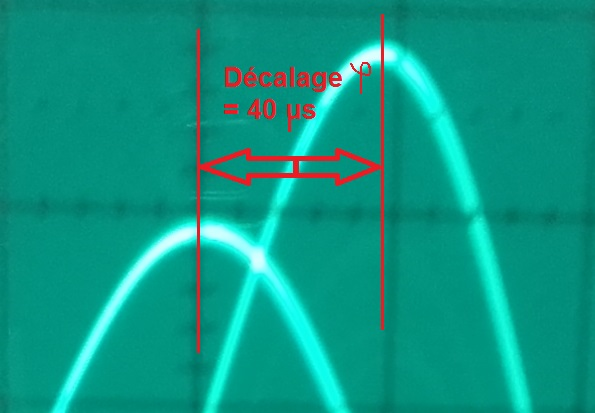
\includegraphics[scale=0.3]{osc3}

\columnbreak

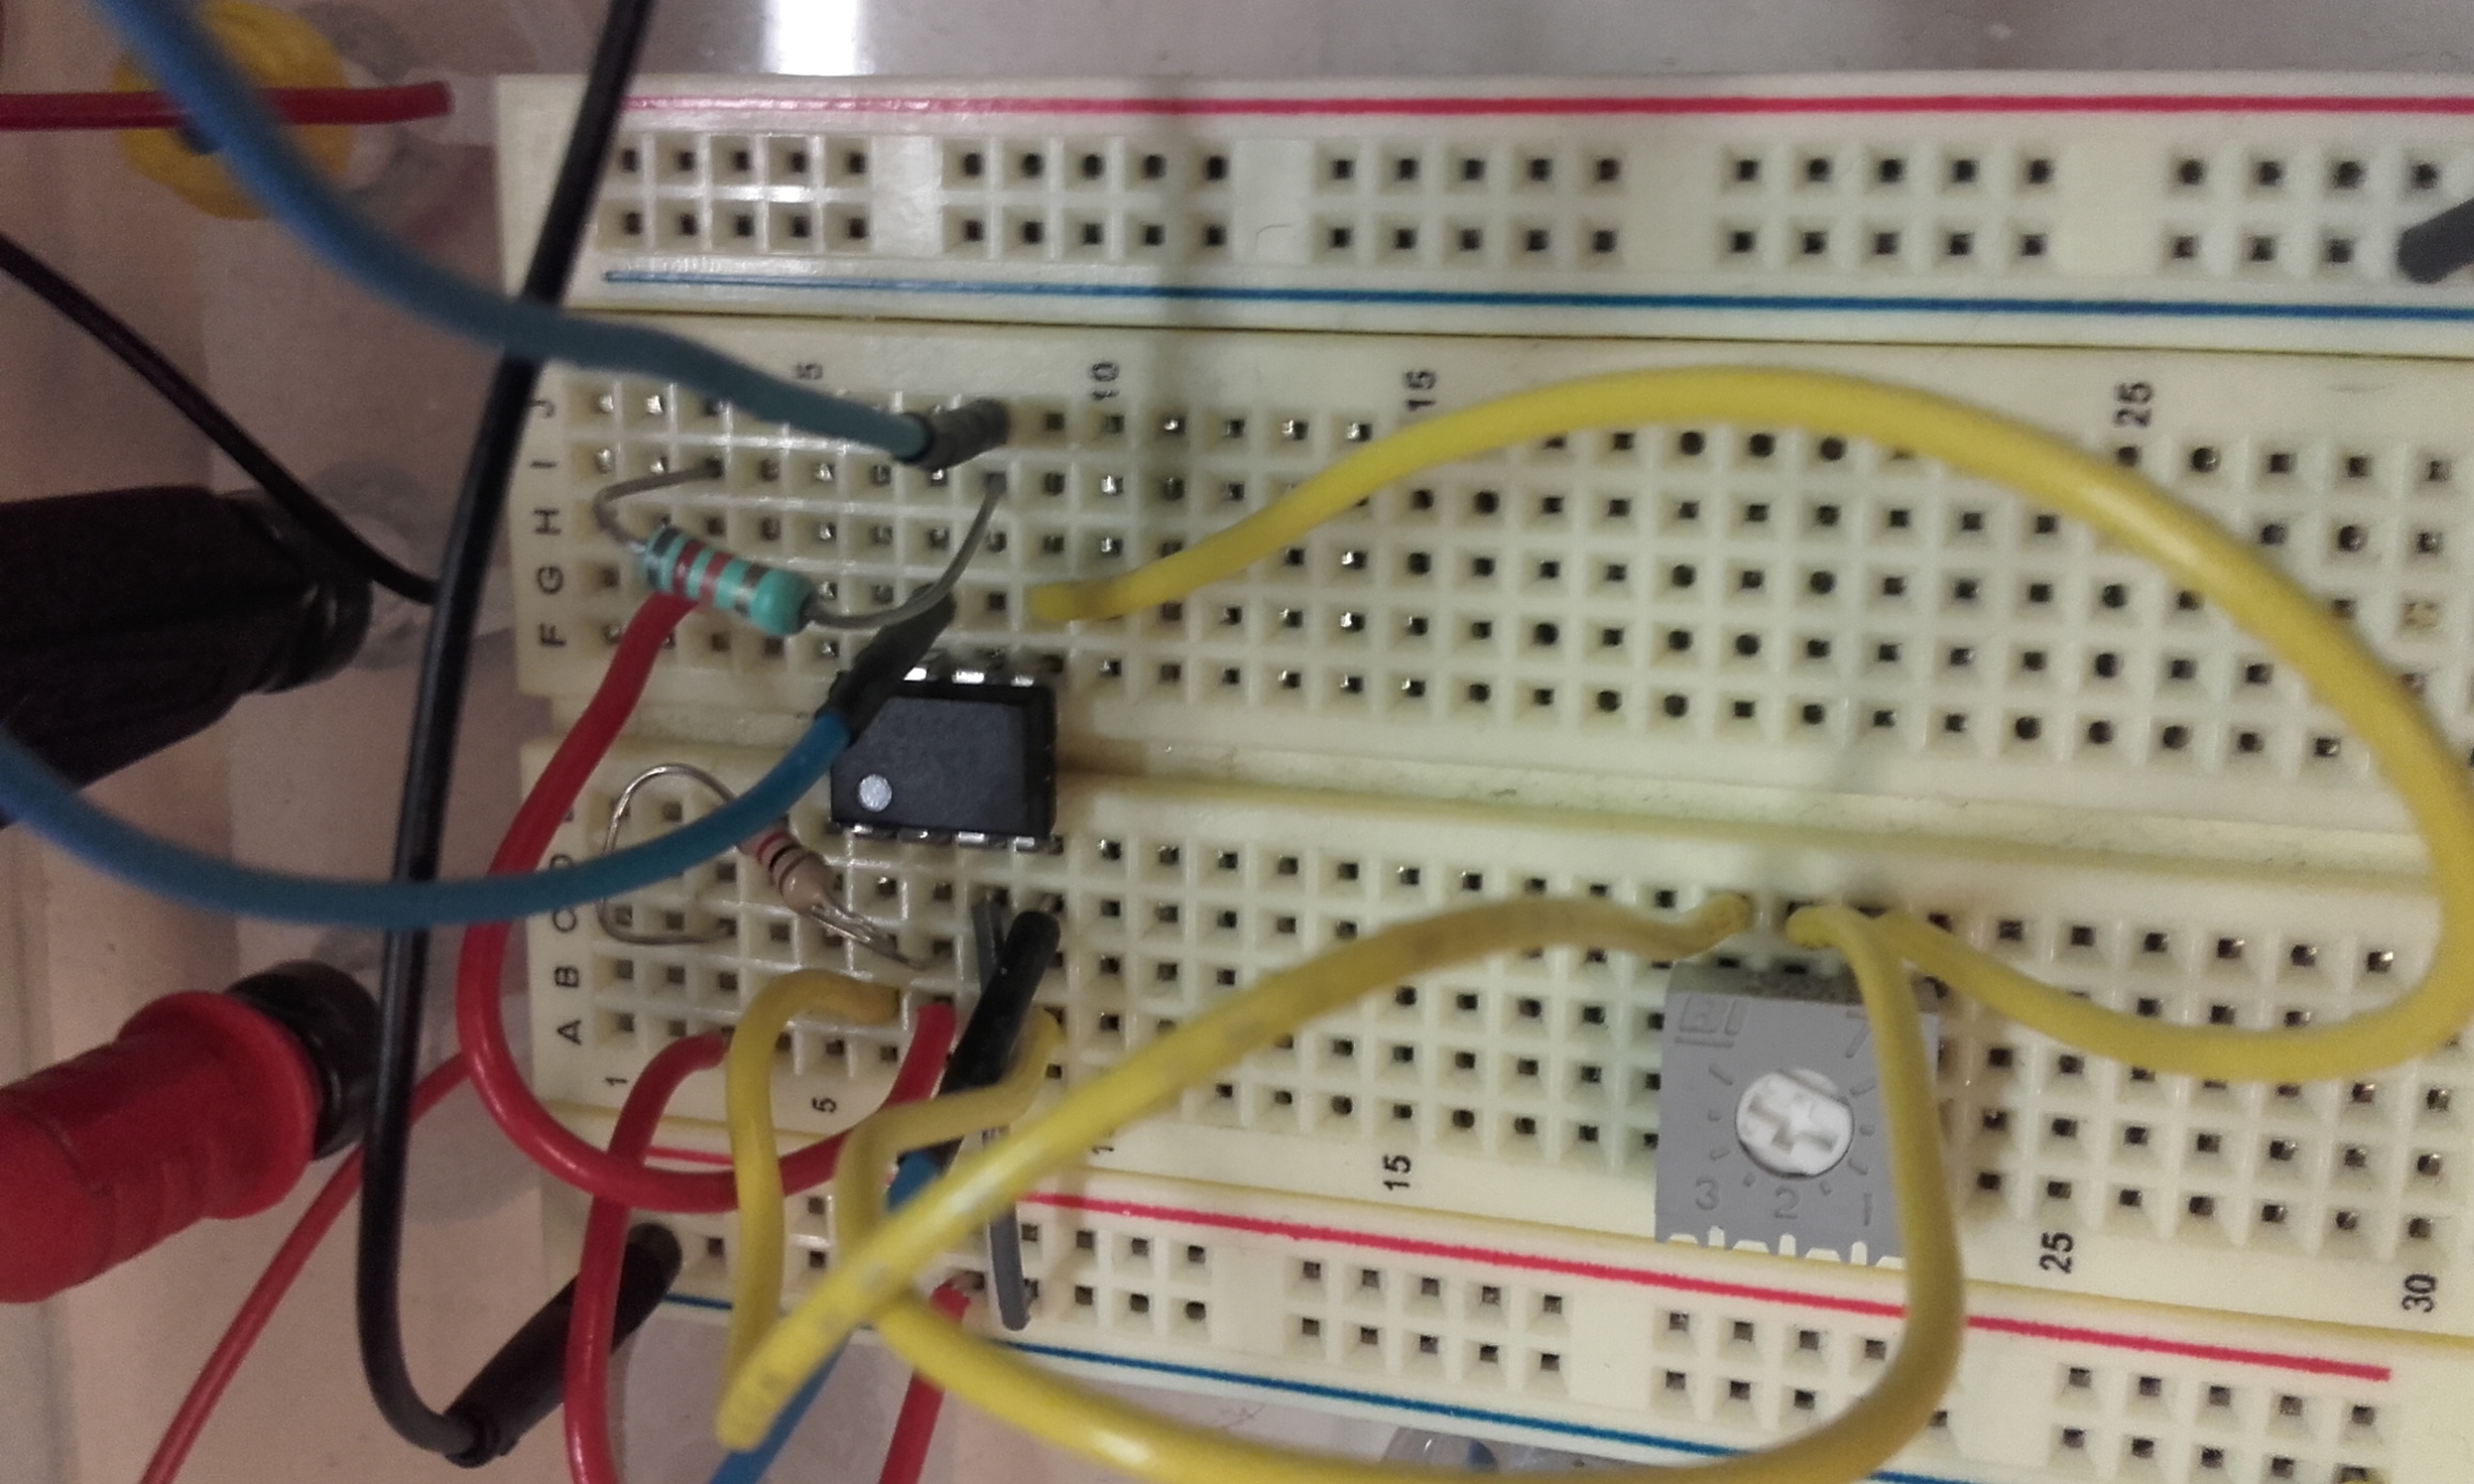
\includegraphics[scale=0.07]{montage1}
\end{multicols}

\vfill\eject

\section{Oscillateur Astable}

\begin{multicols}{2}
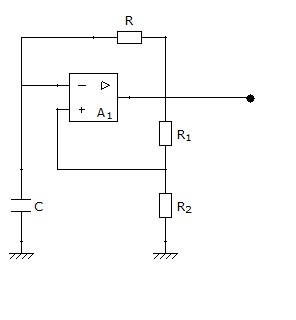
\includegraphics[scale=0.6]{circuit1}

\columnbreak

Avec comme composants : \\
- R = 5.6 $k \Omega$\\
- $R_1$ = 1.2 $k \Omega$\\
- $R_2$ = 1.0 $k \Omega$\\
- C = 470 nF\\

\end{multicols}

\begin{multicols}{2}

Théoriquement, nous devons observer en tension de sortie quelque chose qui \\ ressemble à ça :

\columnbreak

Expérimentalement nous trouvons ça :

\end{multicols}

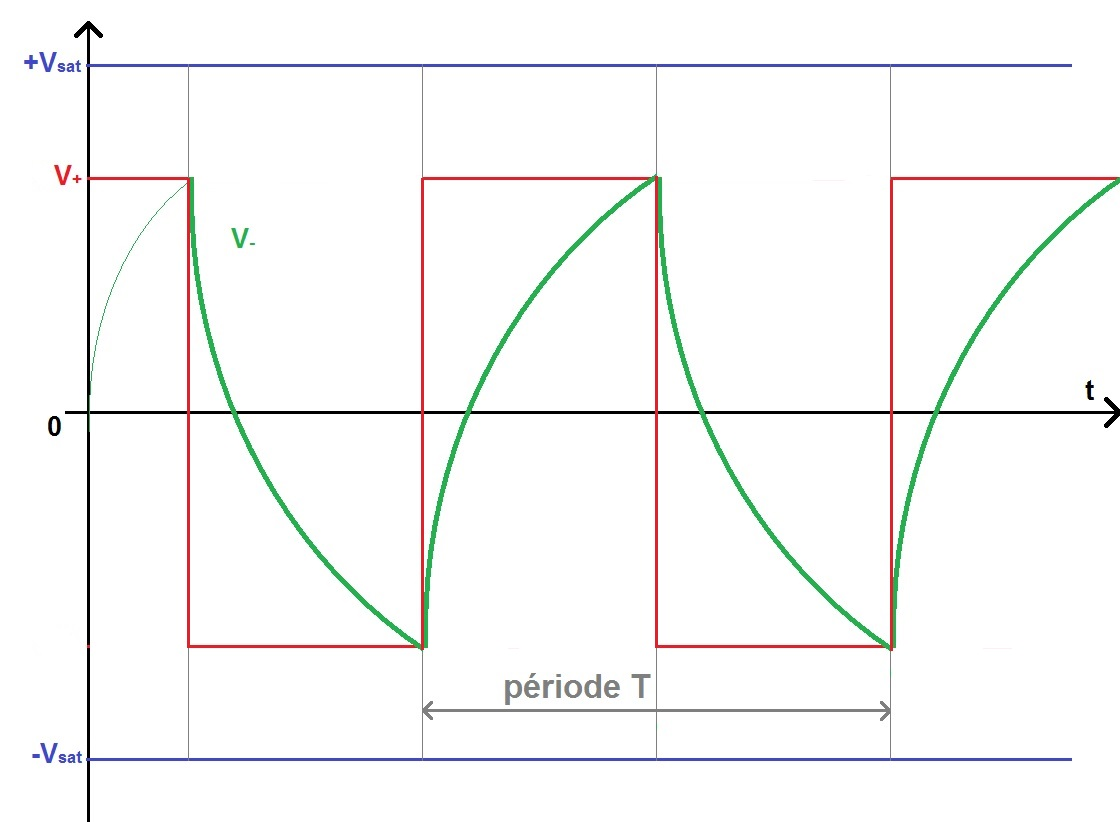
\includegraphics[scale=0.3]{oscastable}
\hspace{1.5cm}
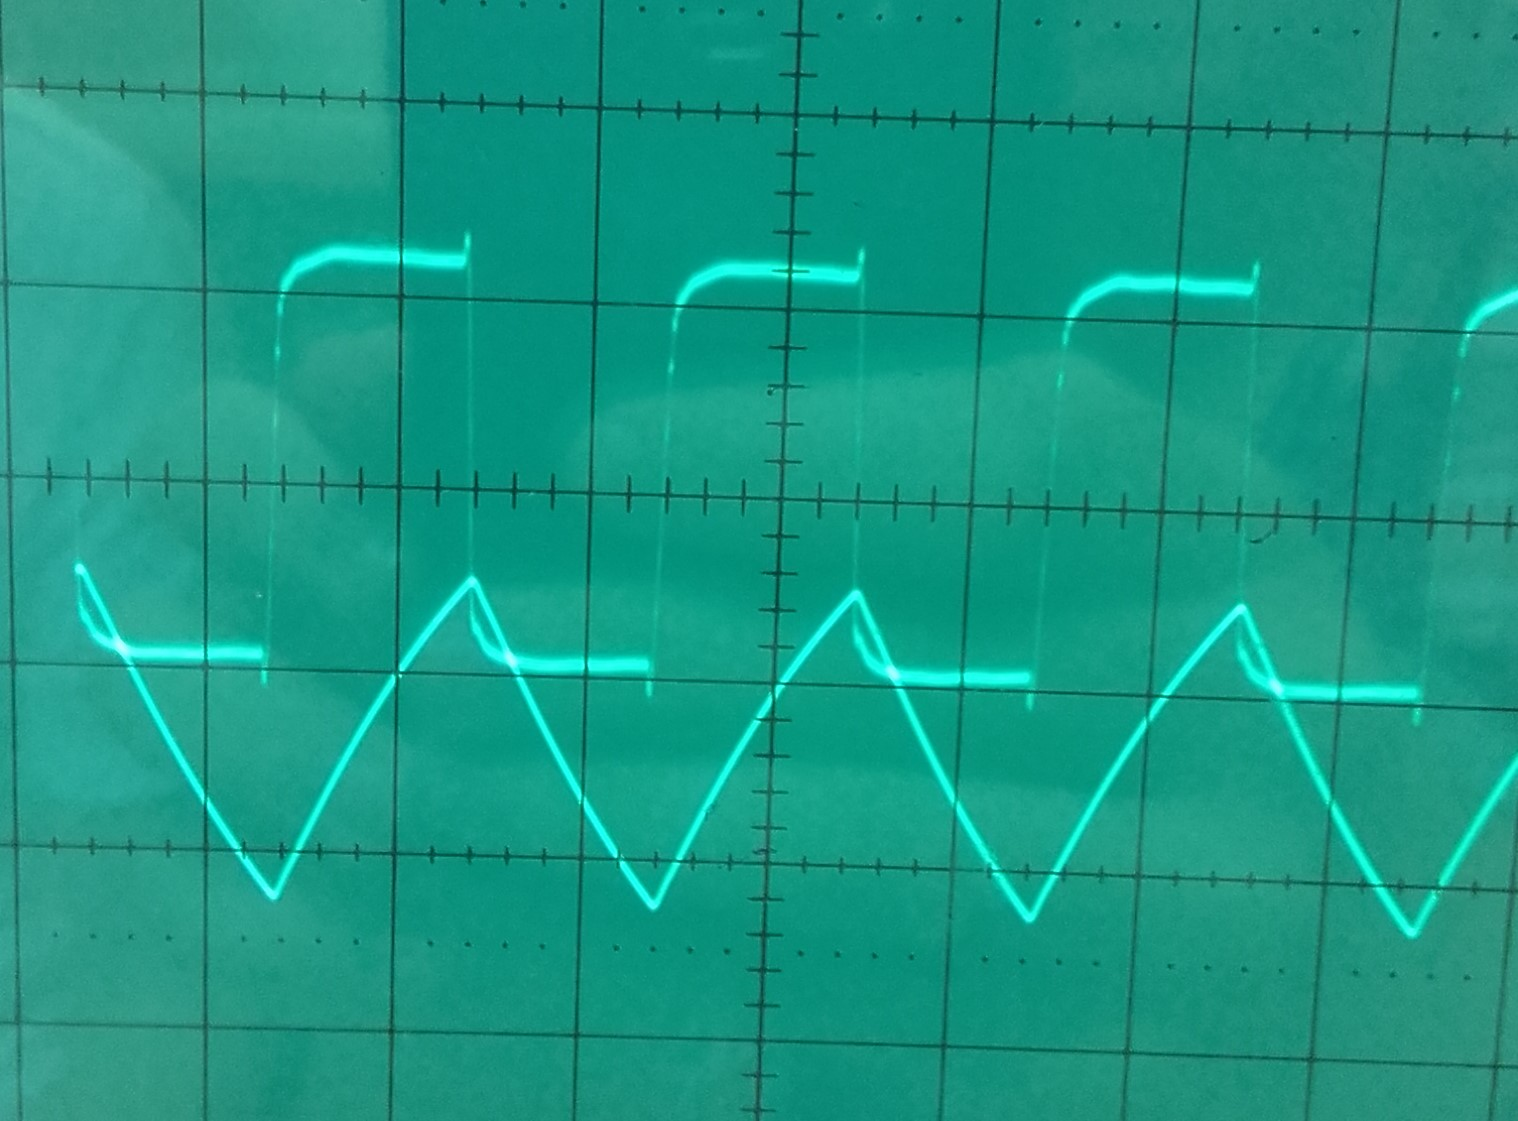
\includegraphics[scale=0.1]{osc1}

On retrouve bien la même forme pour le signal de aux bornes du condensateur ($v_-$) et pour le signal de sorti (signal en "créneaux" arrondi) 
Remarque : les deux signaux ont été décalés pour faciliter des lectures précédentes mais correspondent bien au graph s'ils sont centrés.\\

Théoriquement, on trouve une période T :
\hspace{1.5cm} $T = 2RC.\ln(1+\frac{2.R_2}{R_1})$\\ \\
AN : $T \approx 2.5,6.10^3 . 470.10^{-9}. \ln(1 + \frac{2}{1,2}) \approx 5,16$ ms\\
Avec une incertitude de :

$\Delta T = T\sqrt{\left(\frac{\Delta R}{R}\right)^2 + \left(\frac{\Delta C}{C}\right)^2 + \left(\frac{\Delta R_1}{R_1}\right)^2 + \left(\frac{\Delta R_2}{R_2}\right)^2 }$\\
$\Leftrightarrow \Delta T \approx 5,16.\sqrt{\left(0.05\right)^2 + \left(0.05\right)^2 + \left(0.05\right)^2 + \left(0.05\right)^2 } \approx 0,52 $\\
$\Rightarrow T \approx 5,16 \pm 0,52$ ms\\
\\
Expérimentalement, avec notre balayage de 2 ms par division, on trouve une période de T = 4 $\pm$ 0,4 ms, on tombe bien sur la valeur théorique.\\
En modifiant le signal d'entré $(v_+ = v_e)$ on fait varier symétriquement l'amplitude de notre oscillation et si l'on modifie la fréquence on modifie cette fois asymétriquement la période T (si F $\nearrow$ alors T$\searrow$).\\

Par opposition aux oscillateurs harmoniques, ce système n'oscille qu'en subissant un changement de contrainte provoqué par le condensateur influençant la tension d'entrée. On peut appeler ce système "oscillateur à relaxation" car la contrainte est périodiquement relâchée et la réponse est identique pour chaque période.

\end{document}

